
\chapter{PENDAHULUAN}

\section{Latar Belakang}
% Tentang Citra digital
Citra digital merupakan citra yang dihasilkan dari pengolahan secara digital dengan merepresentasikan citra secara numerik dengan nilai-nilai diskret. Suatu citra digital dapat direpresentasikan dalam bentuk matriks dengan fungsi f(x,y) yang terdiri dari M kolom dan N baris. Perpotongan antara baris dan kolom disebut pixel \thecite{book:gonzalez}. Setiap pixel mewakili sebuah warna, pada citra biner sebuah pixel hanya berwarna hitam atau putih saja. Pada citra grayscale warna sebuah pixel mewakili tingkat keabuannya. Sedangkan pada citra warna (RGB) setiap piksel mewakili warna yang merupakan kombinasi dari tiga warna dasar.

Pada umumnya warna dasar dalam citra RGB menggunakan penyimpanan 8 bit untuk menyimpan data warna, yang berarti setiap warna mempunyai gradasi sebanyak 255 warna . Dewasa ini, citra digital dapat menggunakan 16 bit untuk menyimpan data warna dasarnya, hal ini menyebabkan semakin banyak gradasi warnanya sehingga citra yang dihasilkan memiliki tingkat warna yang jauh lebih banyak. Namun tentu saja hal ini mengakibatkan ukuran file citra digital yang dihasilkan juga menjadi semakin besar walaupun dengan resolusi yang sama.

% Pengolahan Citra digital
Pengolahan citra digital adalah


% Deteksi Tepi dan Algoritmanya, sejarahnya juga sedikit
% Deteksi tepi merupakan salah satu metode dalam pemrosesan cira digital untuk deteksi fitur dan ekstraksi dengan mengidentifikasi titik-titik (pixel) dalam citra yang mengalami perubahan tingkat keabuan secara derastis dan mengalami diskontinu. Salah satu tujuan deteksi tepi yaitu untuk mengurangi jumlah data secara signifikan dalam suatu gambar dan mempertahankan sifat strukturalnya untuk pemrosesan citra lebih lanjut (\cite{rashmi}).

% Berbagai macam metode deteksi dapat digunakan untuk mendeteksi tepi pada citra. Setiap teknik memiliki keunggulan dan karakteristiknya masing-masing. Suatu teknik deteksi tepi mungkin dapat bekerja sangat baik dalam suatu aplikasi tertentu namun sebaliknya belum tentu dapat berjalan secara maksimal pada aplikasi lainnya.

% Manfaat pengolahan citra digital
Manfaat dari pengolahan citra digital antara lain

% Filter Spasial
Filter Spasial adalah
% Filter Linear dan non linear

% Stream Video adalah
Video stream dapat dipandang sebagai serangkaian citra digital berturut-turut \thecite{thesis:jin}. Berbeda dengan format video lainya, video stream ini tidak disimpan pada media penyimpanan sebagai file video melainkan langsung disalurkan setiap framenya dari sumber (source) ke penerima, dalam hal ini FPGA.  Dengan menganggap Video stream adalah kumpulan citra digital (frame) maka dapat dilakukan metode pengolahan seperti pada citra digital, termasuk filter spasial. Setiap citra yang ditangkap dari source disebut sebagai frame, setiap frame ini dilakukan deteksi tepi kemudian hasilnya ditampilkan secara berkesinambungan sehingga nampak seperti video yang telah difilter. 

Frame per second (FPS) atau Frame rate adalah banyaknya frame yang ditampilkan dalam setiap detik pada video. Semakin tinggi FPS sebuah video maka semakin halus pula gerakan yang dapat ditampilkan karena dibentuk dari frame yang lebih banyak, namun dengan jumlah frame yang lebih besar tentu dibutuhkan juga resource yang lebih besar dalam pengolahan video tersebut \thecite{pdf:marcin}. 
% Dalam penelitian ini video stream yang digunakan dibatasi 30 fps saja dengan resolusi 720p.


% FPGA sebagai alat untuk implementasi
Field Programmable Gate Arrays atau FPGA adalah perangkat semikonduktor yang berbasis \textit{matriks configurable logic block} (CLBs) yang terhubung melalui interkoneksi yang dapat diprogram. FPGA dapat diprogram ulang dengan aplikasi atau fungsi yang diinginkan setelah \textit{manufacturing}. Fitur ini yang membedakan FPGA dengan \textit{Application Specific Integrated Circuits} (ASICs), yang dibuat khusus untuk tugas tertentu saja \thecite{XILINX}.

FPGA Xilinx PYNQ-Z2 yang digunakan pada penelitian ini secara official dapat menerima input video stream dari port HDMI Input dengan resolusi maksimal 720p. Video hasil deteksi tepi yang ditampilakan melalui port HDMI Output akan mengalami penurunan fps, hal ini disebabkan oleh penambahan jeda waktu komputasi untuk deteksi tepi antara setiap frame. Setiap frame yang diterima dari \textit{source} akan dilakukan metode deteksi tepi, kemudian hasilnya disalurkan melalui HDMI output untuk kemudian ditampilkan.


% Masalah Performa dan komputasi

\section{Rumusan Masalah}

\section{Batasan Masalah}

\section{Tujuan Penelitian}

\section{Manfaat Penelitian}




\begin{afigure}
    \label{fig:figure2}
    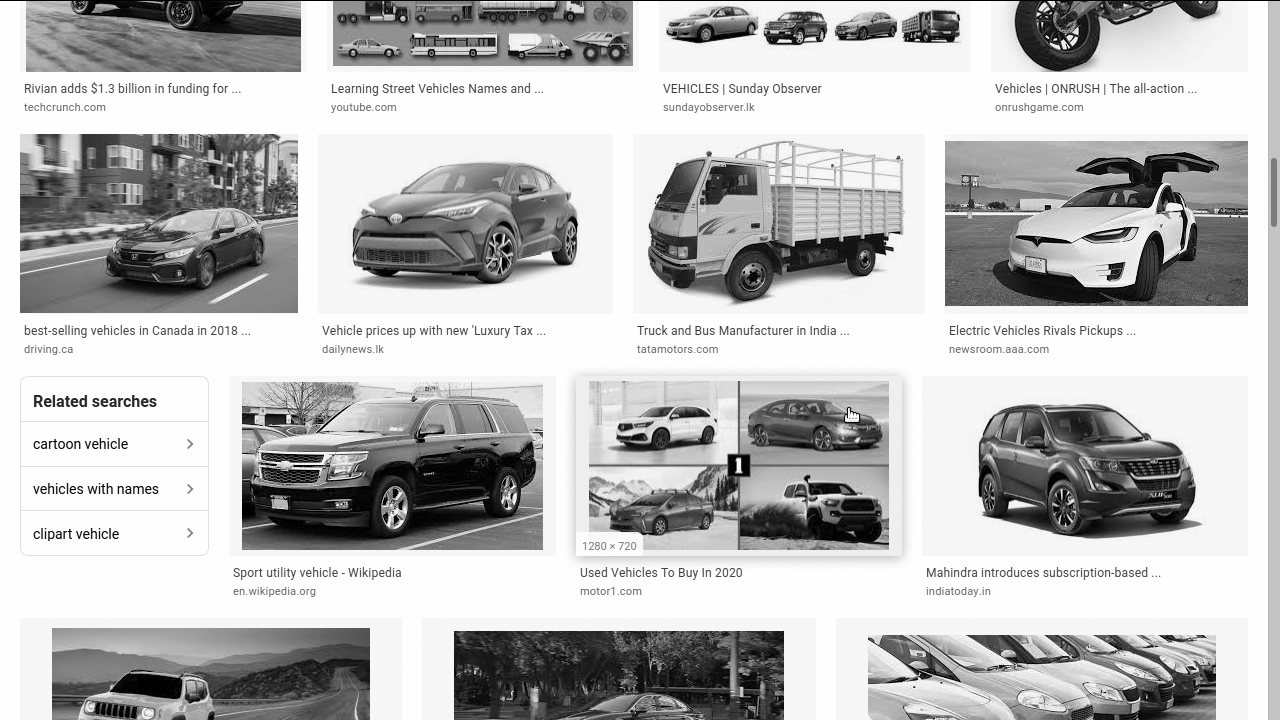
\includegraphics[width=0.5\textwidth, center]{images/input.png}
    \caption{Sebuah gambar}
\end{afigure}

\begin{atable}{Ini Caption tabel}
    \label{table:tabl}
    \begin{tabular}{|l|l|l|l|l|}
    \hline
    fad  & dfaf & fdsfdfads & fdasf & fda  \\
    \hline
    fdas & fdas & ss        & ss    & ss   \\
    \hline
    ss   & dfa  & dfsa      & fdsa  & fdsa \\
    \hline
    ddd  & fdd  & dda       & da    & da \\
    \hline
    \end{tabular}
\end{atable}


\begin{afigure}
    \label{fig:f1}
    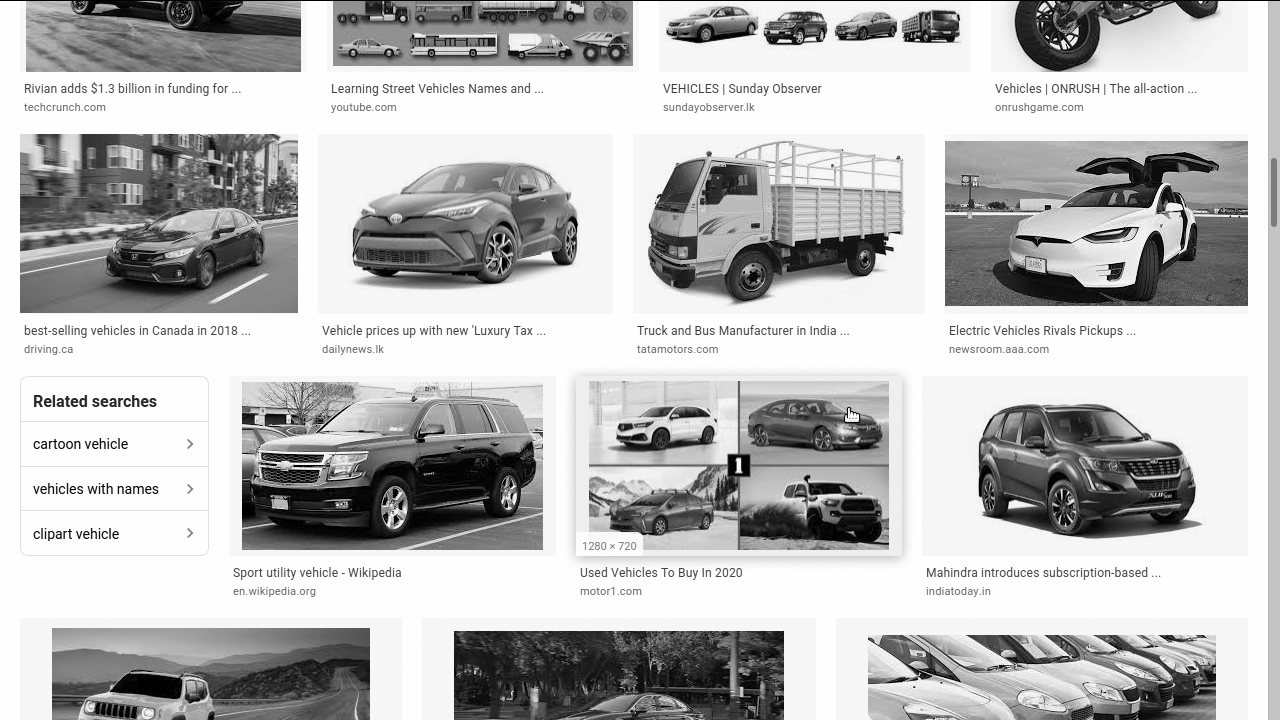
\includegraphics[width=0.5\textwidth, center]{images/input.png}
    \caption{ini gambar na}
\end{afigure}
